
\documentclass[draft]{agujournal2019}
\usepackage{url} %this package should fix any errors with URLs in refs.
\usepackage{lineno}
\usepackage[inline]{trackchanges} %for better track changes. finalnew option will compile document with changes incorporated.
\usepackage{soul}
\linenumbers


\draftfalse



\journalname{Journal of Advances in Modeling Earth Systems (JAMES)}


\begin{document}



\title{The Community Land Model, version 5: \\ Parameter Perturbation Experiment}



\authors{D. Kennedy \affil{1}, Katherine Dagon\affil{1}, David M. Lawrence\affil{1}}
%R.A. Fisher
%B.M. Sanderson
%C.D. Koven
%A.L.S. Swann
%C.M. Zarakas
%L.R. Hawkins
%F. Hoffman
%N. Collier
%Y. Luo
%X. Lu
%S. Levis
%S.C. Swenson
%K.W. Oleson
%E. Kluzek
%J. Liu





\affiliation{1}{Climate and Global Dynamics Laboratory, NCAR, Boulder, CO, USA.}


\correspondingauthor{Daniel Kennedy}{djk2120@ucar.edu}



\begin{keypoints}
\item enter point 1 here
\item enter point 2 here
\item enter point 3 here
\end{keypoints}



\begin{abstract}
[ enter your Abstract here ]
\end{abstract}







\section{Introduction}
\section{Experiment Description}
\label{methods}
\subsection{Model description}
\label{sect:md}
The Community Terrestrial System Model (CTSM) is developed by the CESM Land Model Working Group (LMWG) and maintained at the National Center for Atmospheric Research (NCAR). This experiment utilizes the Community Land Model configuration of CTSM, version 5.1 (CLM5.1). The model source code and documentation are available online (\url{https://github.com/ESCOMP/CTSM}), as is a full model description \cite{lawrence2019}.

Relative to CLM5.0, version 5.1 includes minor bug fixes, several parameter adjustments, and the implementation of biomass heat storage \cite{swenson2019}. The PPE experiment required additional code modifications to identify and programmatically vary the full suite of model parameters. The exact model code for this experiment is contained in a development tag (\url{https://github.com/ESCOMP/CTSM/tree/branch_tags/PPE.n11_ctsm5.1.dev030}). We utilized the full biogeochemistry version of CLM in land-only mode, with the crop model turned off. The component set longname is: \\ \texttt{2000\_DATM\%GSWP3v1\_CLM51\%BGC\_SICE\_SOCN\_SROF\_SGLC\_SWAV\_SIAC\_SESP}

\subsection{Model spin-up}
Model spin-up for the equilibration of carbon and nitrogen pools within biogeochemistry-enabled land models can consume up to 98\% of computational time \cite{sun2023}. Depending on the evaluation criteria and model configuration, CLM5 requires between 800 and 2000 years (or more) to reach steady-state conditions \cite{lawrence2019}. Absent equilibrium, the drift towards steady state can obscure important model dynamics or features. For this reason, each member of the PPE requires independent spin-up.

To manage computational cost we leveraged the Matrix-CN spin-up mode recently implemented within CLM \cite{lu2020}. This new module leverages a linearized simplification of CLM's biogeochemistry to significantly reduce spin-up time. Our spin-up protocol featured 20 years in accelerated decomposition mode, followed by 80 years of Matrix-CN, followed by 40 years of `normal' mode, cycling over a ten-year forcing dataset. This was designed to achieve sufficiently equilibrated model states, while minimizing computational time. To reduce model cost, we did not require full equilibration of deep soil carbon (beyond 1 meter). Any inferences about deep soil carbon would therefore be subject to uncertainty due to spin-up concerns.

\subsection{Sparsegrid}
\label{sect:sg}
One of the largest controls on model cost is resolution. Most CLM simulations utilize nominal 1$^\circ$ resolution, which requires over 20,000 land grid cells. In order to manage computational cost, parameter perturbation experiments often use lower resolution, such as 4$^\circ$x5$^\circ$ \cite{dagon2020}. CLM does not require standard rectilinear grids, which allows for innovative techniques to reduce model resolution

Multivariate spatio-temporal clustering (MVSC) has been utilized to extract patterns of climatological significance from climate model output \cite{hoffman2005} and applied to design a representativeness-based sampling network \cite{hoffman2013}. Instead of lowering resolution by increasing grid spacing, we used MVSC to strategically remove redundant grid cells, leaving only 400 grid cells that efficiently sample important model dynamics. Our goal was to quantify parameter effects with sufficient accuracy, while minimizing computational cost.

We used k-means clustering to identify groups of grid cells with similar climatologies based on a 2$^\circ$ transient simulation (1850-2014) using the CLM-PPE codebase. Instead of running every grid cell from a given cluster, we only run one representative grid cell, whichever is located nearest the cluster centroid in climate space. We refer to the set of representative grid cells as the `sparsegrid'. A paint-by-number approach is used to recompose mapped output and compute global means, where the output from the representative grid cell is substituted for all members of the cluster cohort.

Clustering was based on a subset of 18 meaningful CLM variables (Table \ref{tab:sg}). The clustering algorithm received 12 observations of each variable per grid cell, namely the mean and interannual variability computed for six 30-year climatology windows (1865-1894, 1895-1924, ... , 1985-2014). Clusters were delineated to equalize the multi-dimensional variance across the user-specified number of groups, $k$. We tested 15 values of $k$, ranging from 10 to 800. Based on ILAMB2.5 benchmarking \cite{collier2018} against the full grid output, we opted for a 400-cluster sparsegrid, to balance computational cost against model fidelity (Supp Figure \ref{supp:ilamb}). Because our emphasis is on vegetated regions, we masked out Antarctica within the clustering algorithm, whereby we do not provide any output below 60$^\circ$S.

\begin{table}[h]
\caption{Clustering inputs}
\centering
\begin{tabular}{l c c c c}
 \hline
 Climate forcing variables & Ecosystem state variables &Ecosystem flux variables \\
 \hline
 2m air temperature (TSA) & Leaf area index (TLAI) & Gross primary production (GPP) \\
Atmospheric rain (RAIN) & Ecosystem carbon (TOTECOSYSC) &Heterotrophic respiration (HR) \\
Atmospheric snow (SNOW) &  Ecosystem nitrogen (TOTECOSYSN) &Autotrophic respiration (AR) \\
2m specific humidity (Q2M) & Soil ice (TOTSOILICE) &Net biome production (NBP) \\
Solar radiation (FSDS) & Soil liquid water (TOTSOILLIQ) & Total liquid runoff (QRUNOFF) \\
& Snow cover fraction (FSNO) & Sensible heat  (FSH) \\
&&Latent heat (EFLX\_LH\_TOT ) \\
 \hline
 \end{tabular}
 \label{tab:sg}
 \end{table}


\subsection{Experimental Design}
493 simulations.
Nine simulations failed.


\subsection{Forcing Scenarios}
\label{sect:exps}
 \begin{table}[h]
 \caption{Forcing Scenarios}
 \centering
 \begin{tabular}{l c c c c}
 \hline
  Name  & Meteorology & CO$_2$ (ppmv) & N addition & Description \\
 \hline
   CTL2010  & 2005-2014 & 367 & - & control experiment\\
   C285        & 2005-2014 & 285 & - & low CO$_2$ \\
   C867        & 2005-2014 & 867 & - & high CO$_2$ \\
   AF1855    & 1851-1860 & 367 & - & pre-industrial climate \\
   AF2095    & 2091-2100 & 367 & - & late century climate (SSP3-7.0) \\
   NDEP      & 2005-2014 & 367 & 5g/m$^2$ & enhanced nitrogen deposition \\
 \hline
 \end{tabular}
 \label{tab:exps}
 \end{table}

\subsection{Analyses}
\section{Results}

\begin{figure}[h]
\centering
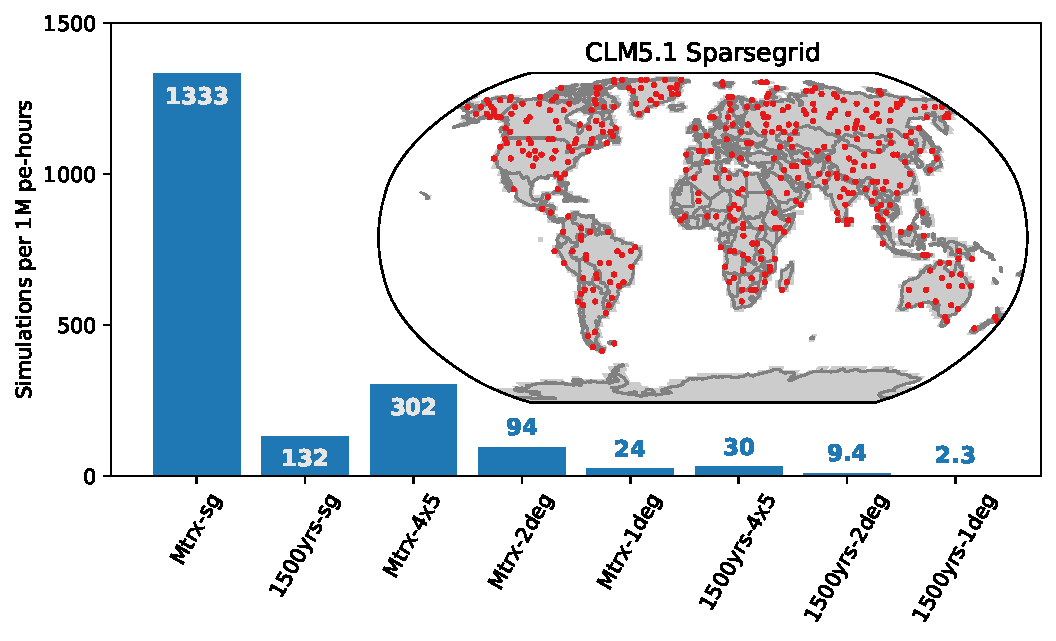
\includegraphics[width=30pc]{../figs/sims.pdf}
\caption{The approximate number of simulations afforded by 1 million core-hours for a range of CLM configurations. Configurations are labeled according to spin-up procedure and resolution, with `sg' signifying sparsegrid. The inset map shows the locations of the 400 sparse grid cells as the red dots. See Section \ref{methods} for spin-up and sparsegrid details. My speed calculations here are a bit janky, assume linear scaling of cost for increasing time or space (zqz). }
\label{fig:sims}
\end{figure}

\begin{figure}[h]
\centering
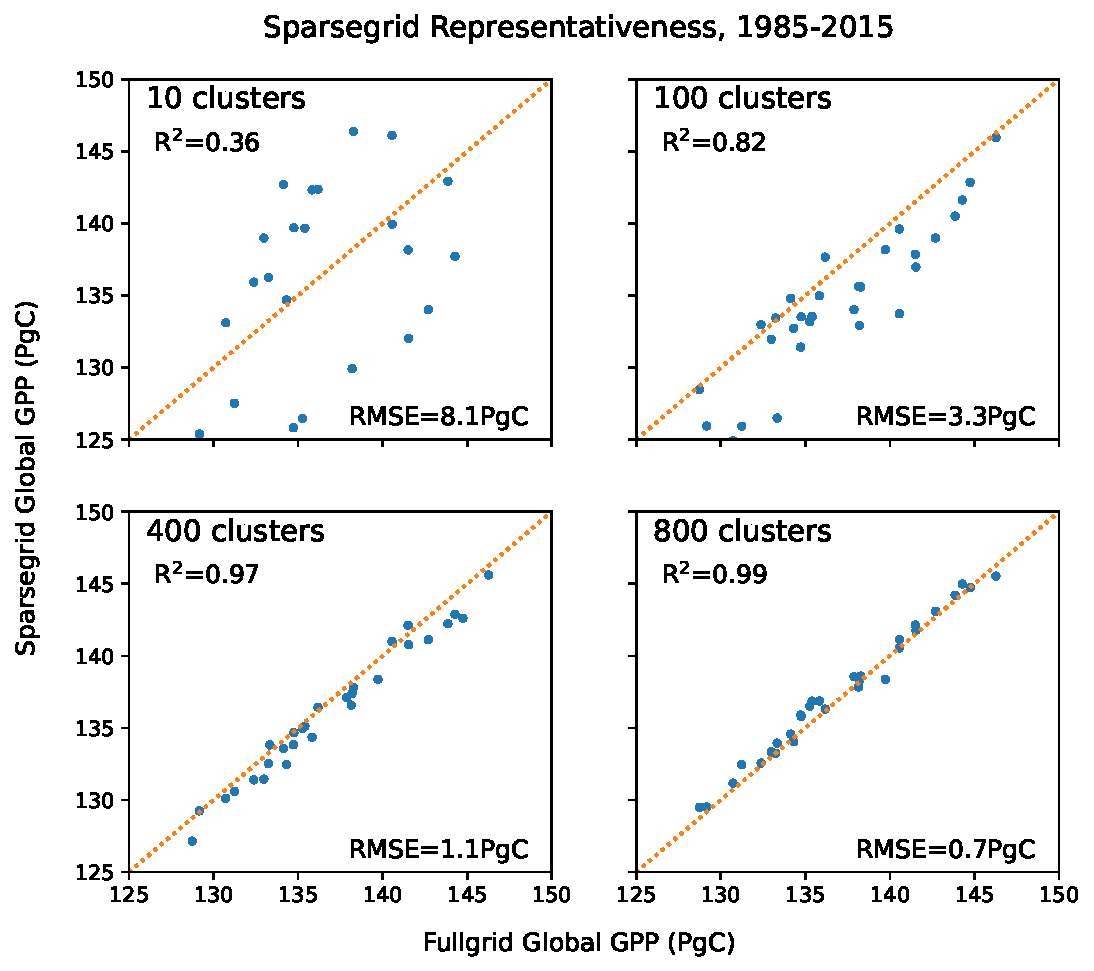
\includegraphics[width=40pc]{../figs/sparsegrid_gpp.pdf}
\caption{Sparsegrid vs fullgrid (2$^{\circ}$ resolution) global annual GPP across the last thirty years of a transient CLM5.1 simulation. We opted for 400 clusters to balance computational cost against representativeness. For reference there are 22648, 5666, and 1764 land gridcells in standard 1$^{\circ}$, 2$^{\circ}$, and 4$^{\circ}$x5$^{\circ}$ CLM simulations, respectively.}
\label{}
\end{figure}

\begin{figure}[h]
\centering
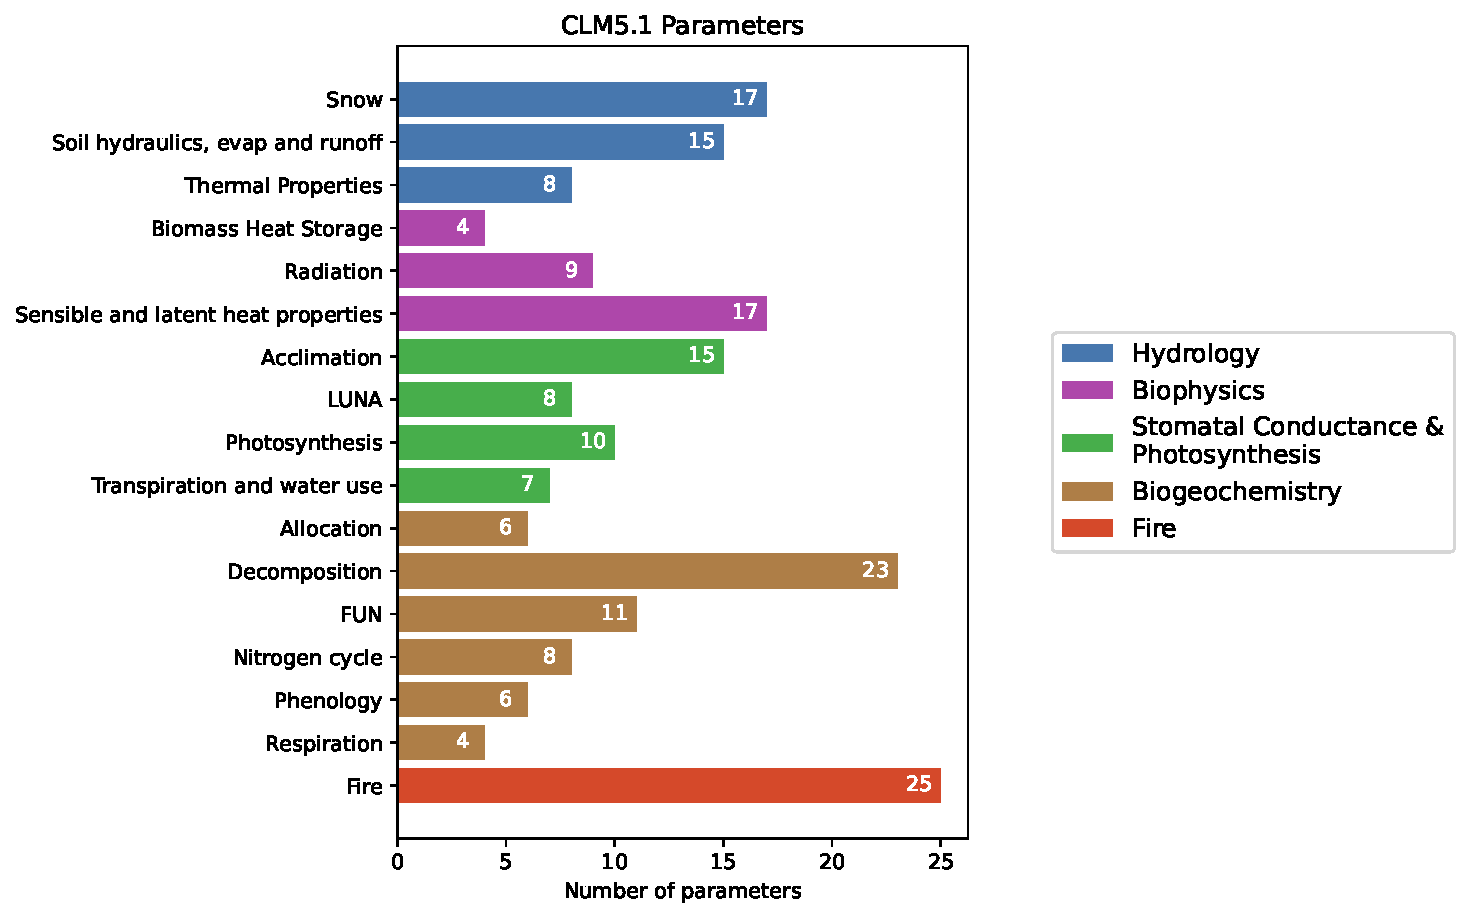
\includegraphics[width=30pc]{../figs/bar.pdf}
\caption{206 parameters were identified and perturbed across the various domains of the land model.}
\label{fig:params}
\end{figure}


\begin{figure}[h]
\centering
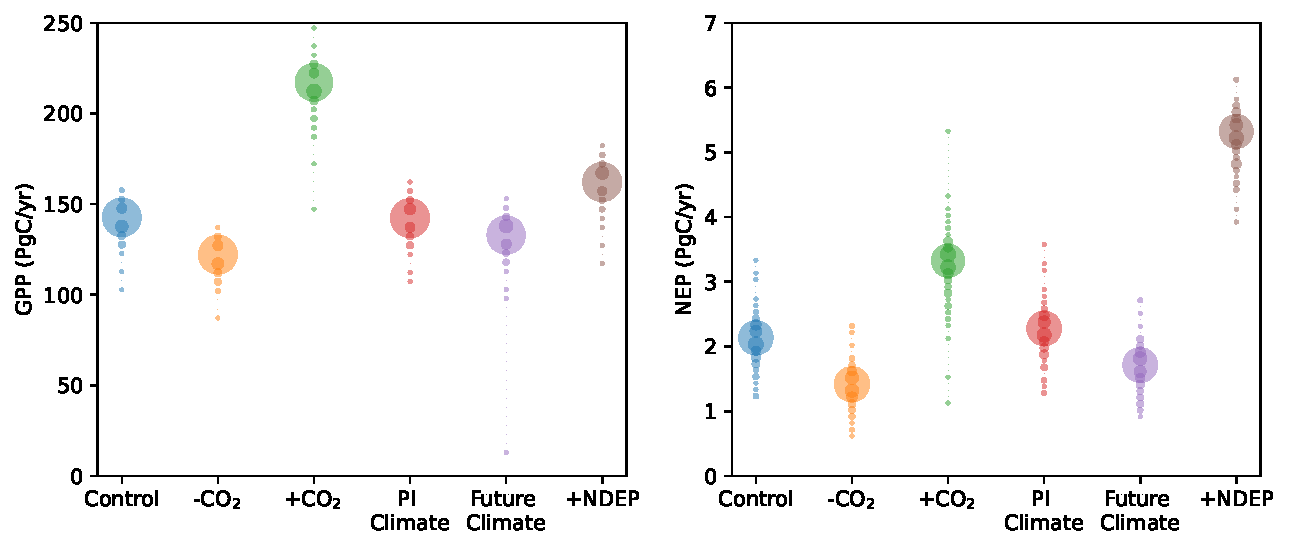
\includegraphics[width=35pc]{../figs/violins.pdf}
\caption{Distributions of global annual gross primary production (GPP) and net biome production (NBP) across the six forcing scenarios. See Section \ref{sect:exps} for scenario descriptions. The distributions are concentrated around the default parameterization with long tails, indicating that a small proportion of parameters have large effects on these two variables. In the case of NBP, parameter effects appear larger than scenario effects.}
\label{}
\end{figure}

\begin{figure}[h]
\centering
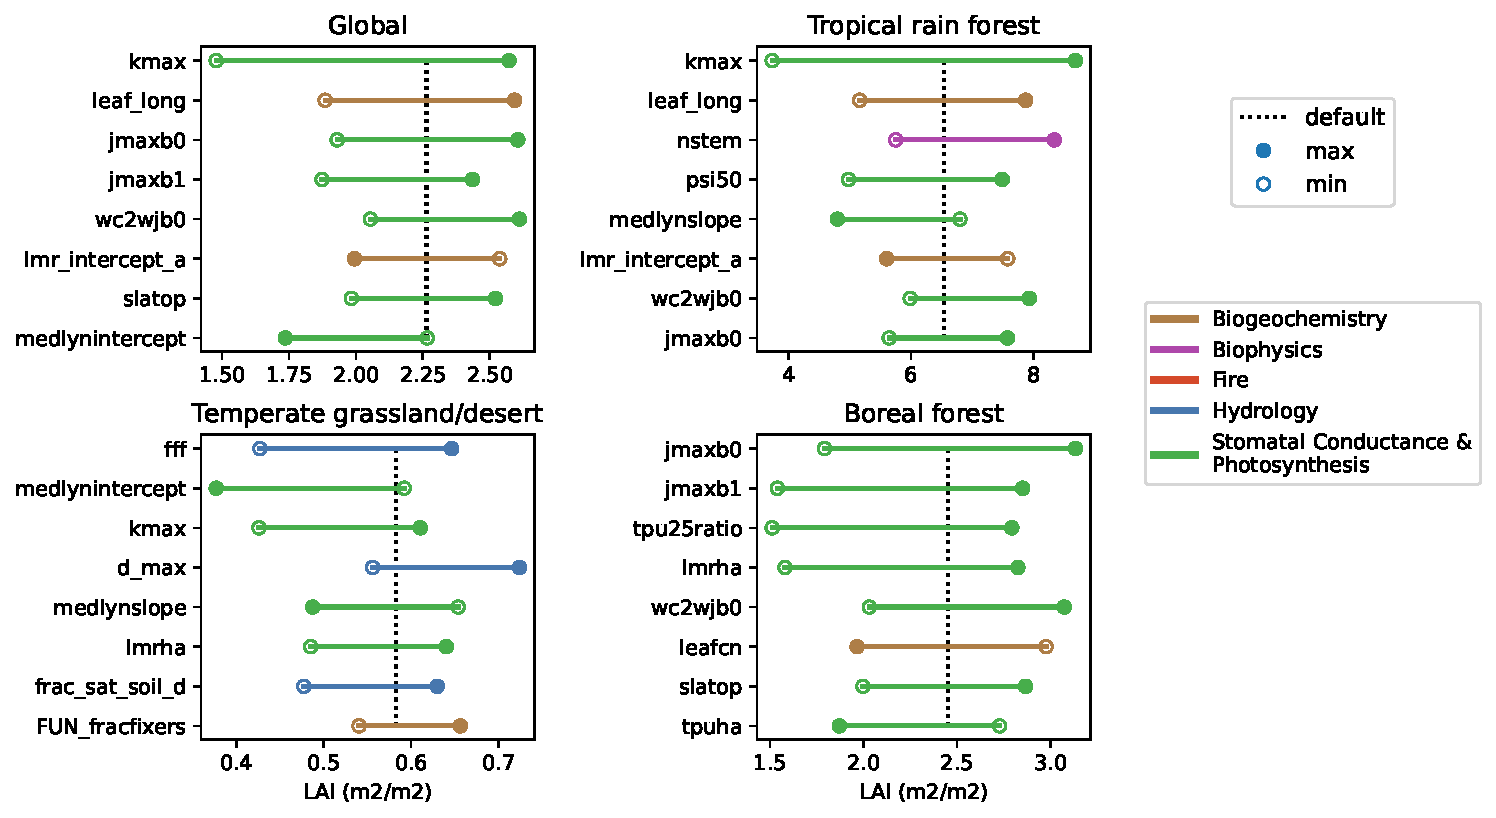
\includegraphics[width=40pc]{../figs/lai_biome.pdf}
\caption{The eight most influential parameters on leaf area index within the CTL2010 ensemble, globally and within three biomes.}
\label{fig:lai}
\end{figure}

\begin{figure}[h]
\centering
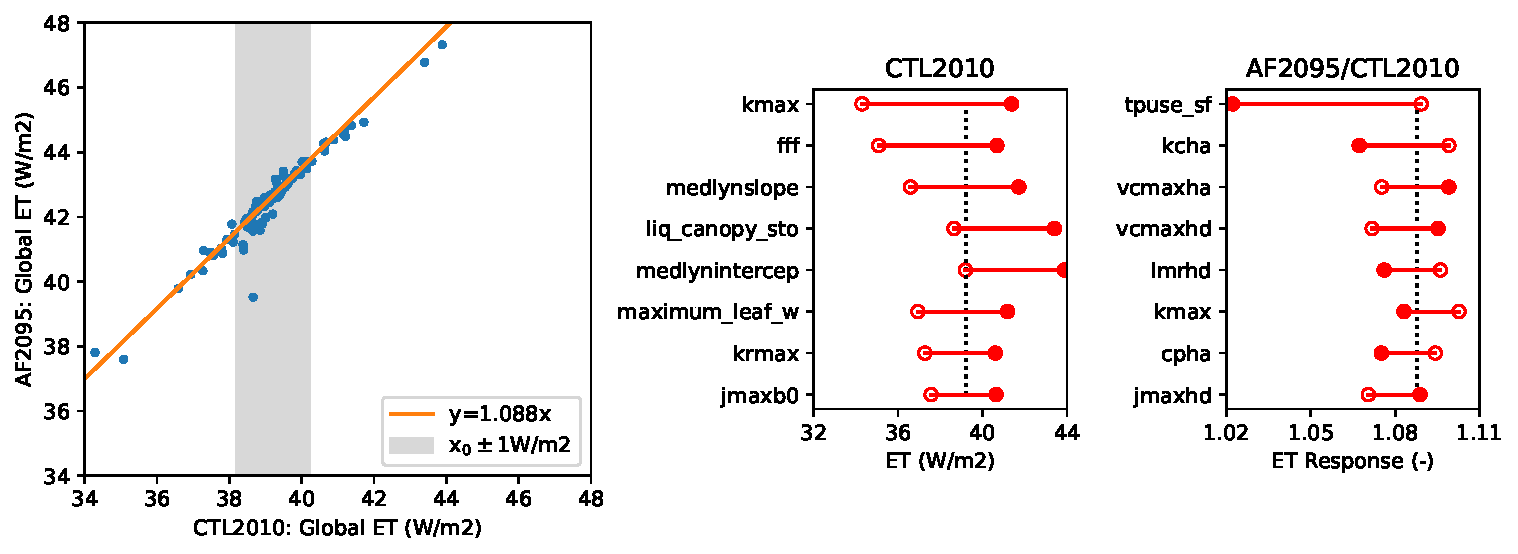
\includegraphics[width=40pc]{../figs/ET_response.pdf}
\caption{(a) Global evapotranspiration in the warm forcing scenario vs. our control experiment. The default parameterization ET enhancement is +8.8\%, as shown with the orange line. The shading spans the CTL2010 default ET, plus or minus 1 W/m2.
(b) The top 8 parameters governing global ET in the CTL2010 experiment.
(c) The top 8 parameters governing ET response to the future climate anomaly forcing (AF2095).
Parameters governing the response to temperature anomalies tend to differ from the parameters controlling present-day ET.}
\label{fig:et}
\end{figure}


\begin{figure}[h]
\centering
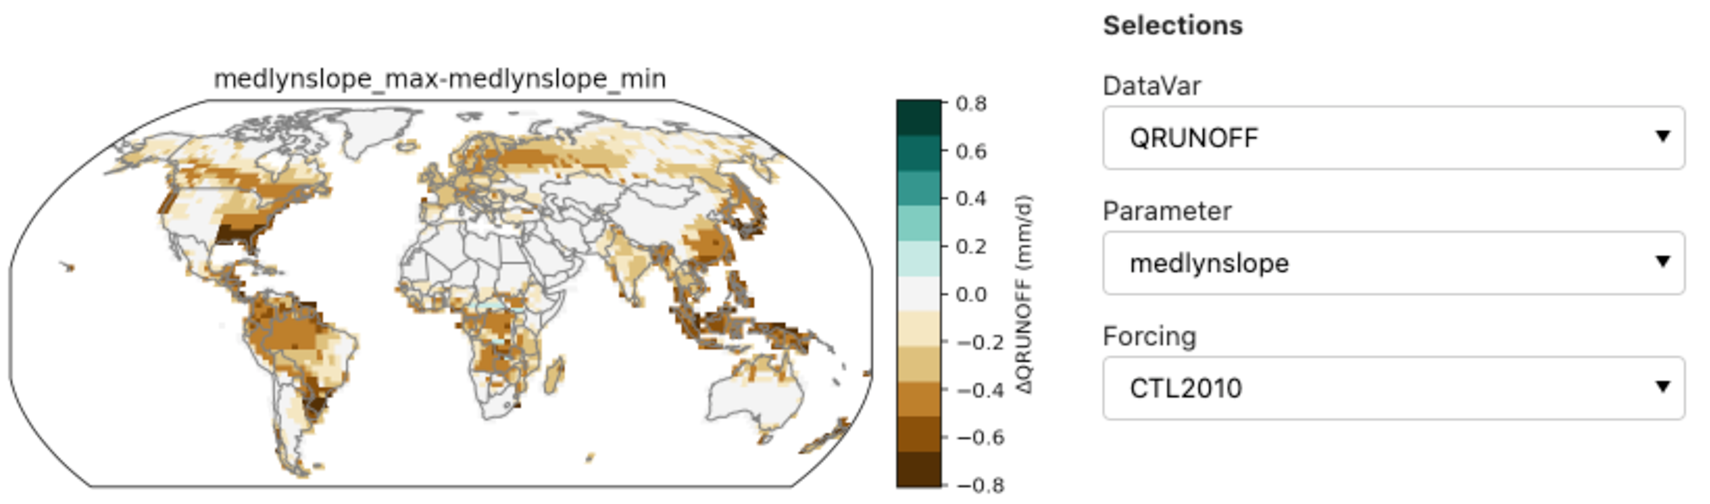
\includegraphics[width=40pc]{../figs/deltmap_panel.pdf}
\caption{Screenshot of interactive diagnostic for exploring maps of parameter effects. In this case, the effect of medlynslope on runoff within the CTL2010 ensemble. Increasing medlynslope tends to increase transpiration and reduce runoff.}
\label{fig:panel}
\end{figure}

\section{Discussion}
\section{Conclusion}
\section*{Open Research Section}
This section MUST contain a statement that describes where the data supporting the conclusions can be obtained. Data cannot be listed as ''Available from authors'' or stored solely in supporting information. Citations to archived data should be included in your reference list. Wiley will publish it as a separate section on the paper’s page. Examples and complete information are here:
https://www.agu.org/Publish with AGU/Publish/Author Resources/Data for Authors


\acknowledgments
Enter acknowledgments here. This section is to acknowledge funding, thank colleagues, enter any secondary affiliations, and so on.




\bibliography{refs}

\appendix
\section{Supplementary Figures}


\begin{figure}[h]
\centering
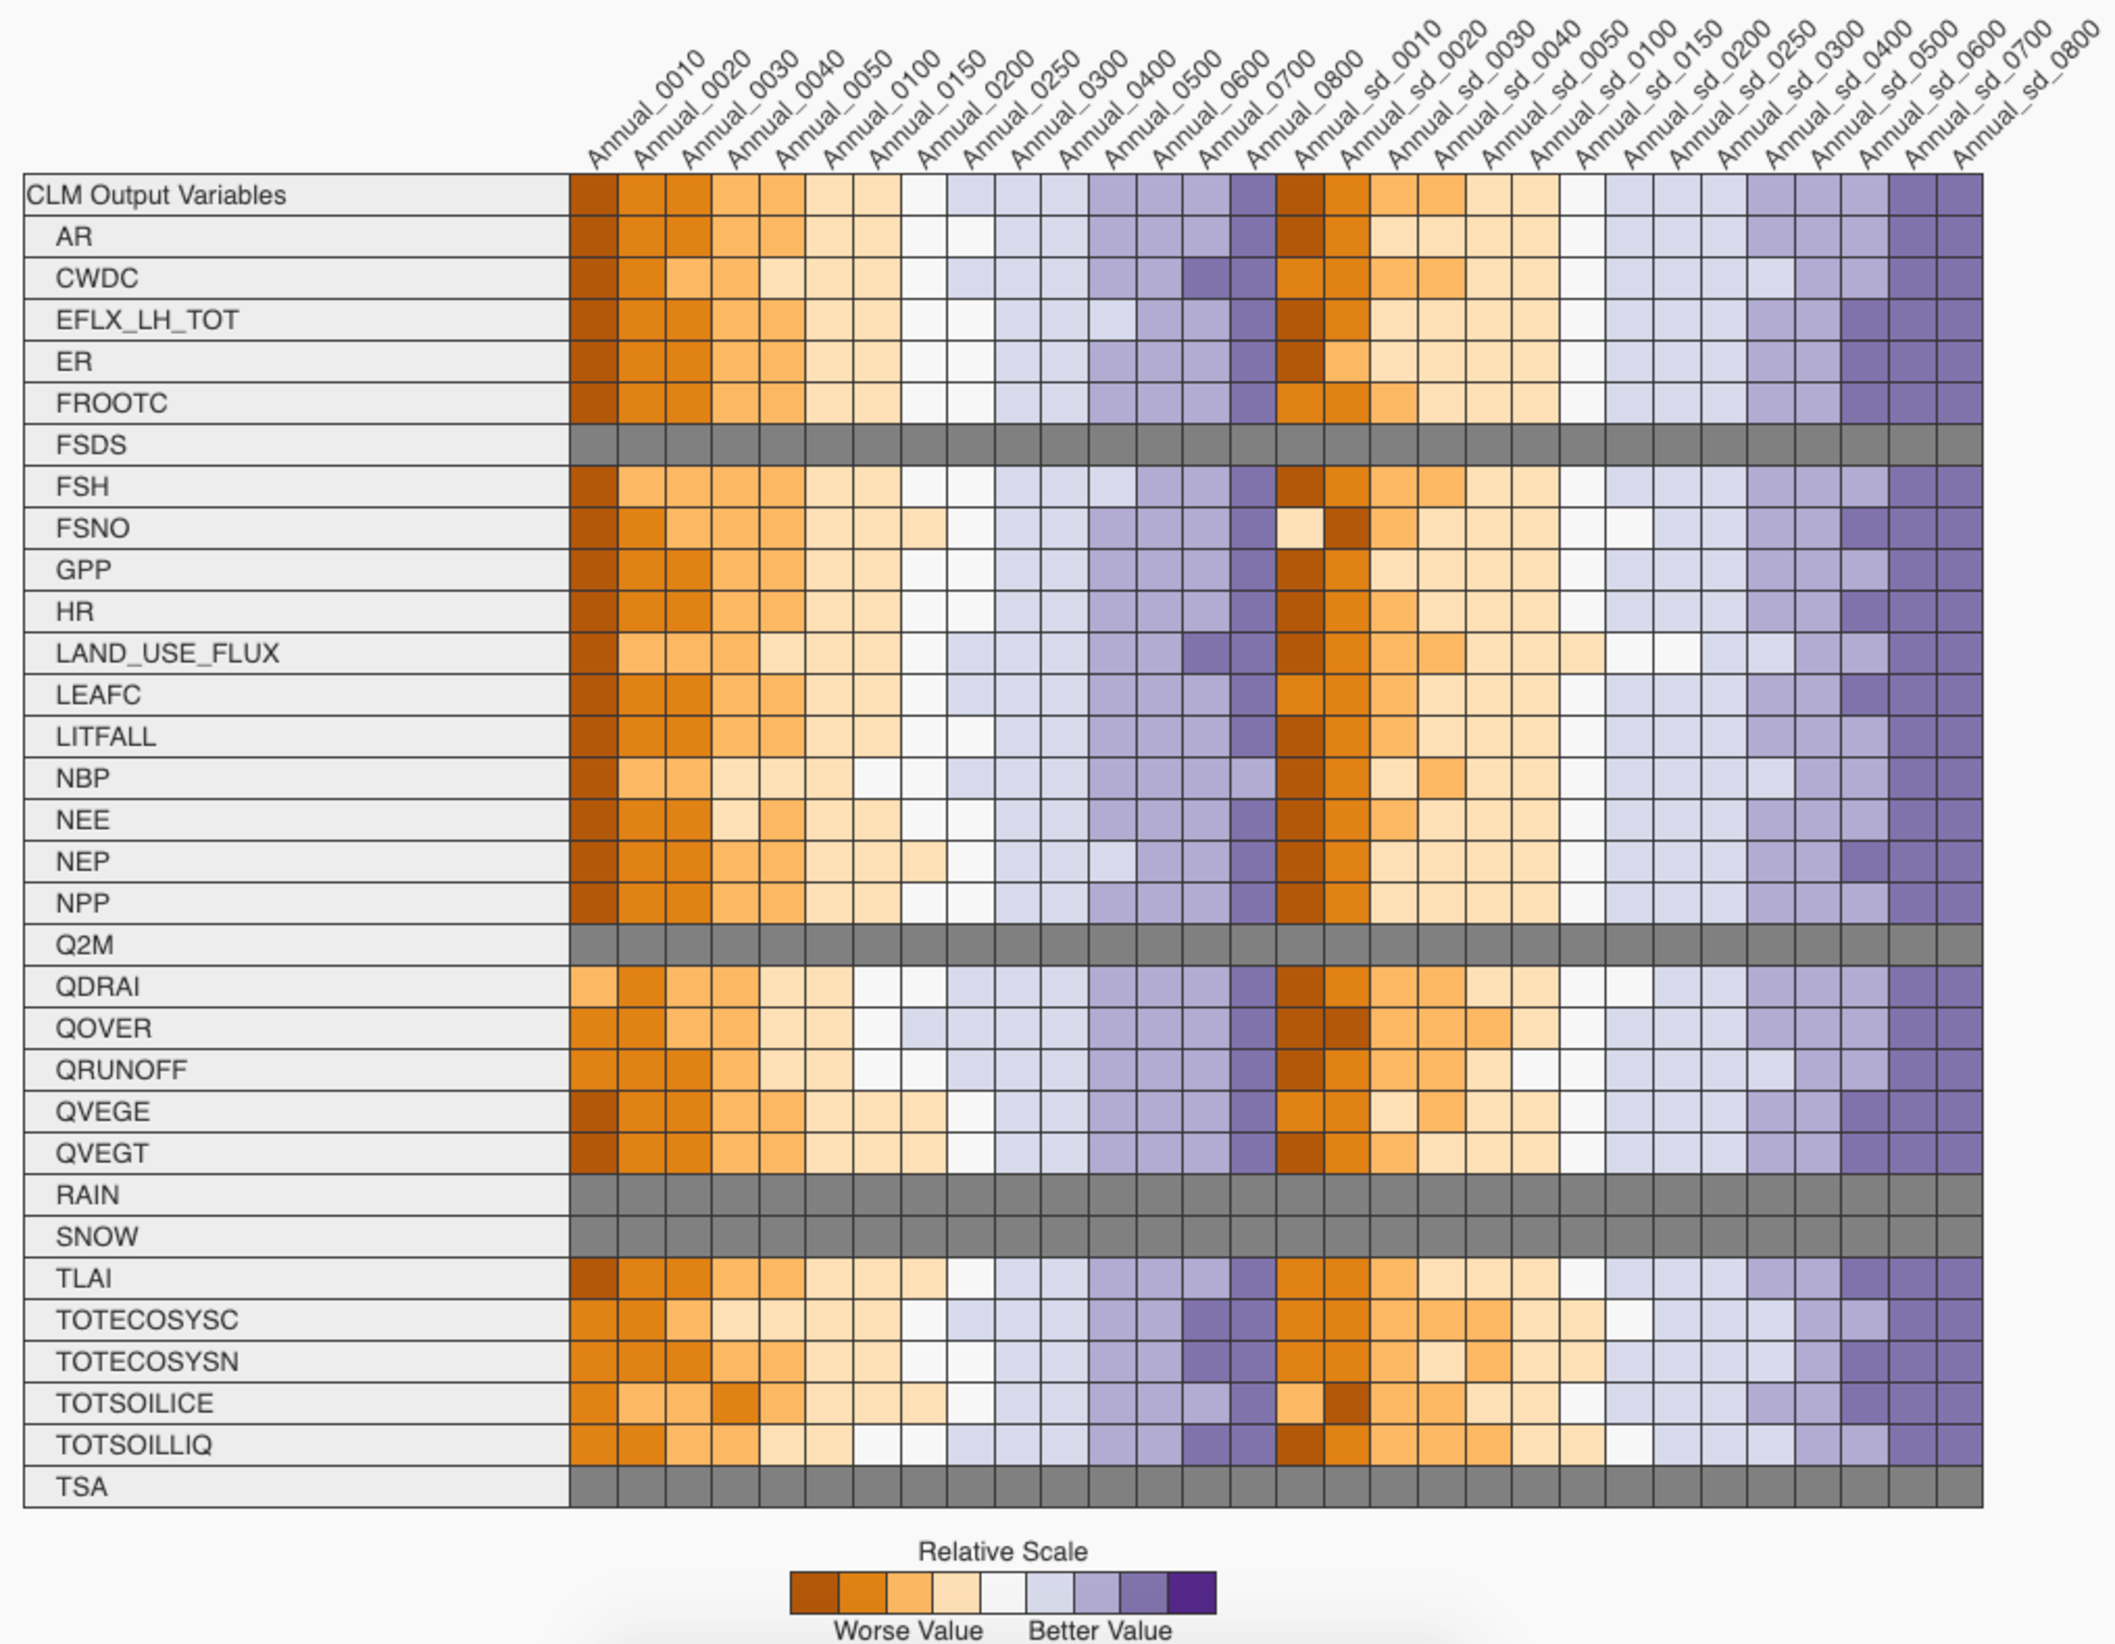
\includegraphics[width=42pc]{../figs/supp/ilamb.pdf}
\caption{ILAMB 2.5 overall scores comparing remapped sparsegrid output to the full grid 2$^{\circ}$ model output. Column headings indicate the number of clusters, and whether annual means or annual means and standard deviations were used as input to the clustering algorithm. We should try to remove the gray bits (zqz). Full, interactive results are available at \url{www.ilamb.org/PPE/CLM/2021-02}. See main text Section \ref{sect:sg} for clustering details.}
\label{supp:ilamb}
\end{figure}



\end{document}




